{
\begin{figure*}[th]
\begin{center}
\centerline{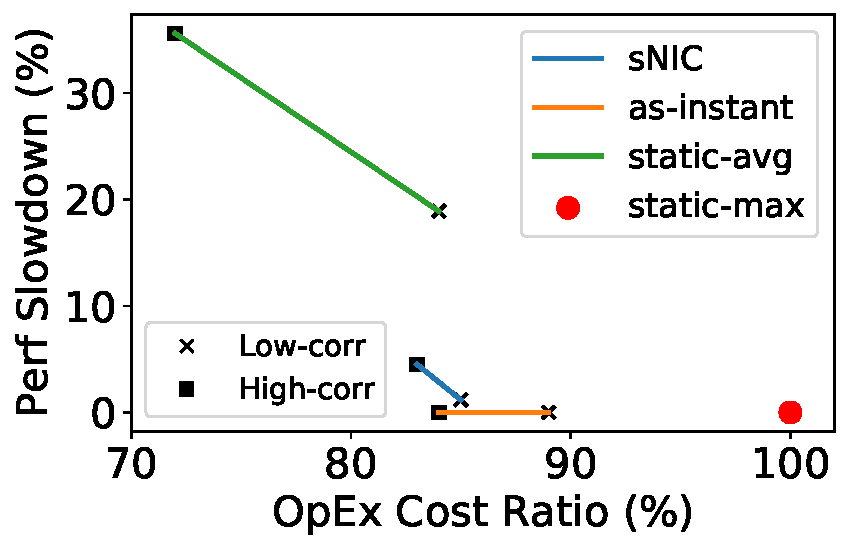
\includegraphics[width=0.5\textwidth]{snic/Figures/fig-conslid-overview-new.pdf}}
\mycaption{fig-sim-overview}{Performance and OpEx Overview.}
{
Lower is better for both axis.
}
\end{center}
\end{figure*}
}
{
\begin{figure*}[h]
\begin{center}
\centerline{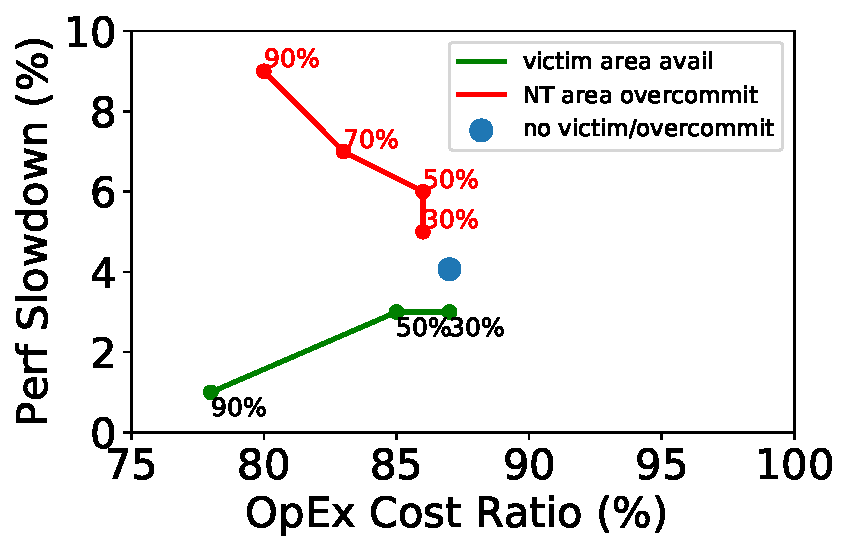
\includegraphics[width=0.5\textwidth]{snic/Figures/fig-single-snic-low-corr.pdf}}
\mycaption{fig-sim-single-snic}{Single \snic{} Sensitivity.}
{
Each lines is running a different set of experiments.
}
\end{center}
\end{figure*}
}
{
\begin{figure*}[h]
\begin{center}
\centerline{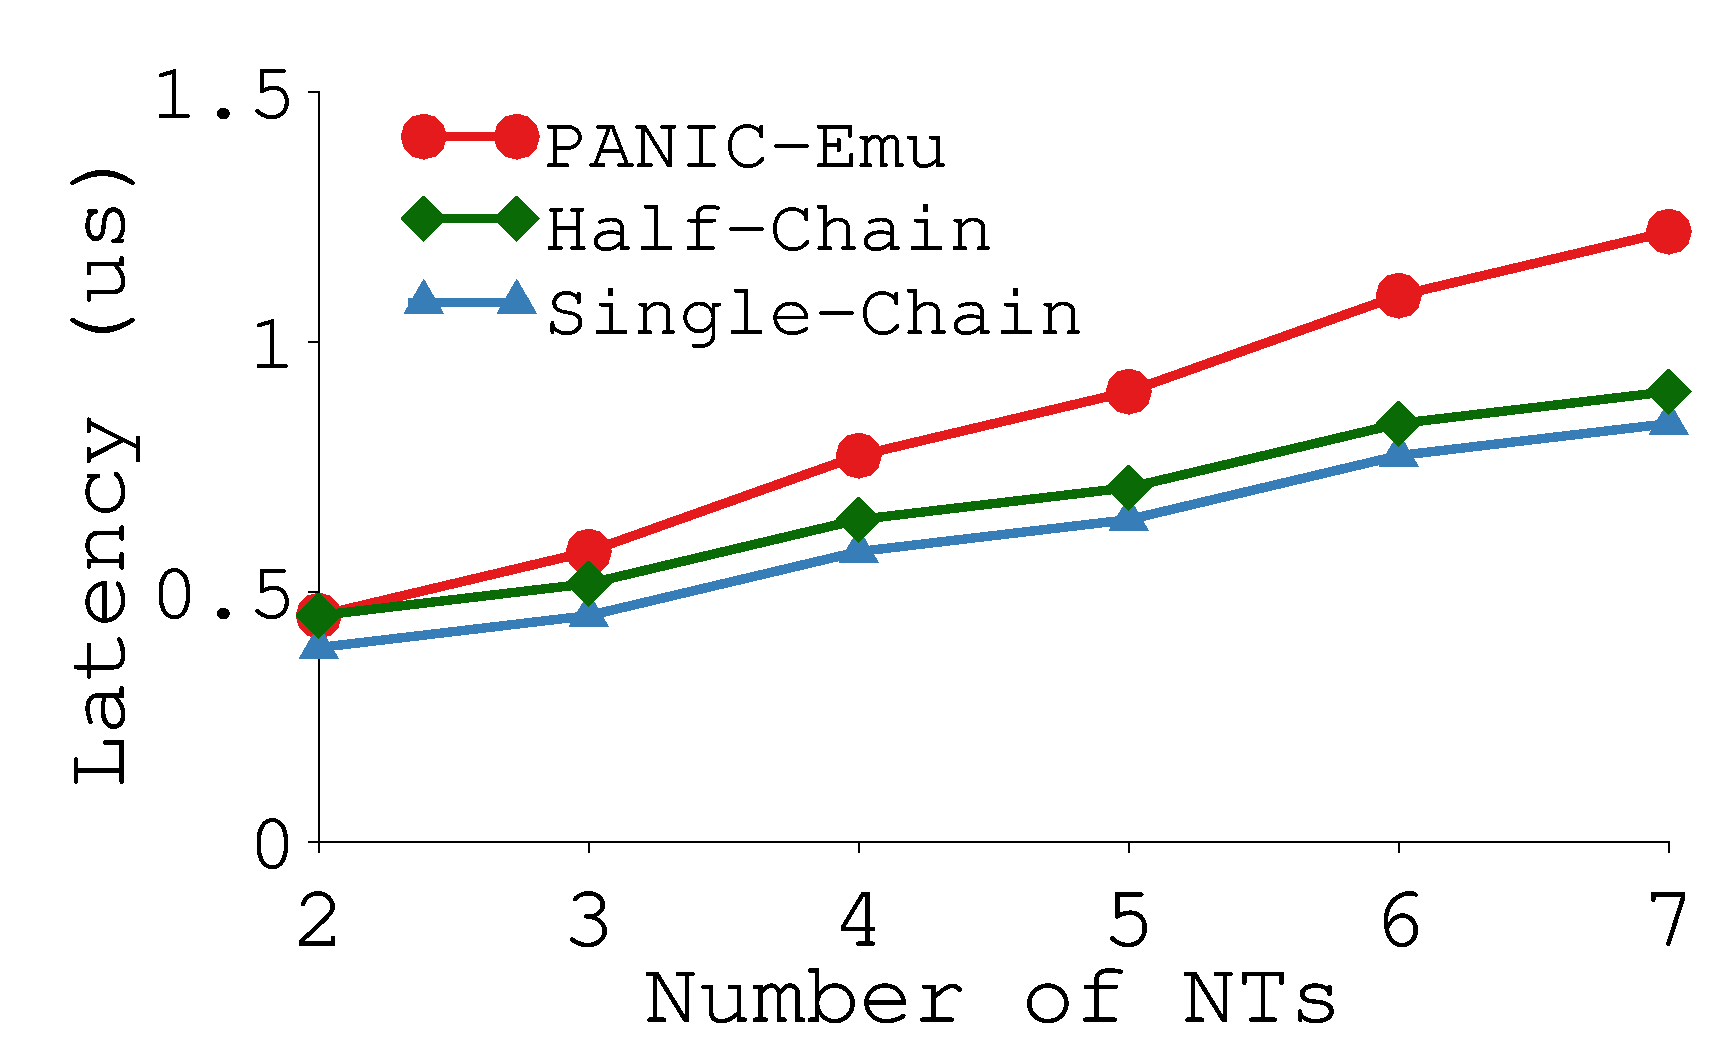
\includegraphics[width=0.5\textwidth]{snic/Figures/g_plot_nt_chain.pdf}}
\mycaption{fig-nt-chain}{\nt{} Chain.}
{
}
\end{center}
\end{figure*}
}
{
\begin{figure*}[h]
\begin{center}
\centerline{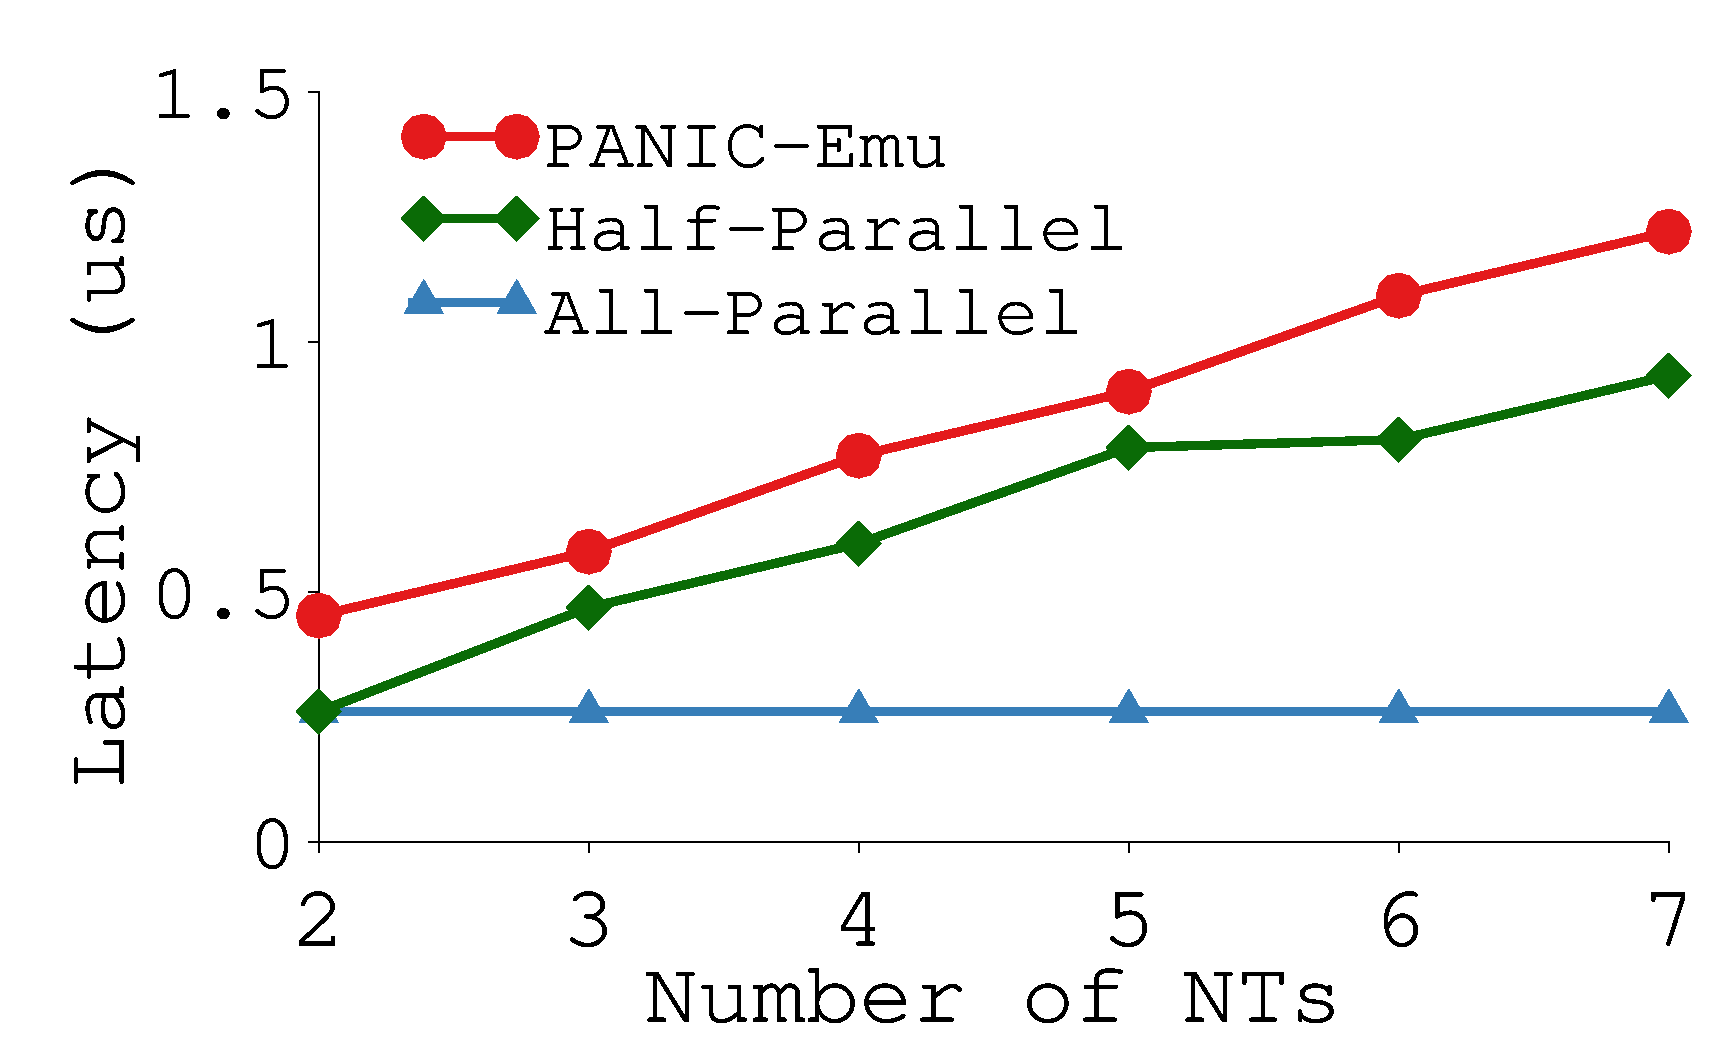
\includegraphics[width=0.5\textwidth]{snic/Figures/g_plot_nt_parallel.pdf}}
\mycaption{fig-nt-parallel}{\nt{} Parallelism.}
{
}
\end{center}
\end{figure*}
}